% !TEX root = ../main.tex

\section{Reconciliation}
\label{sec:reconc}

\subsection{Absolute Direction}
\label{sec:reconc_dir}

One way to interpret state-level political direction is as a proxy for the political belief of the average resident. Under this interpretation, the negative coefficients on STDIR in \Cref{tab:3} suggest that Democratic belief are associated with higher stock market participation (SMP) rates. This finding appears to contradict the individual-level evidence that Republicans are more likely to hold stocks \citep{kaustia2011, ke2024}. 

However, subsampling the data at the state level reveals a different story. Treating the state-level political contribution measure as a proxy for individual beliefs misinterprets the data, and this divergence is an example of Simpson's paradox. \Cref{tab:7} reports the coefficients $\beta_STDIR$ from the \Cref{tab:7} \subref{tab:7a} column 2 regressions, estimated on each state separately. That is, the reported values are the marginal effect of the state-level political direction variable on the probability of stock market participation, holding state and individual characteristics constant. 

The coefficients in \Cref{tab:7} are essentially the time-series effect of the political direction variable within each state, as STDIR(N) has one value per state-year combination. Considering how STDIR(N) was constructed as the percentage of Republican versus Democratic contributors, the time-series variation in this variable can be seen as the change in individual political preferences within the state.


% --- Table 7 ---
% --- PAGE 1: PANEL A ---
\begin{sidewaystable}[htbp]
    \centering
    \caption{Stock Market Participation and State Politics By State}
    \label{tab:7}
    \small 

    \begin{minipage}{\textheight}
        This table presents the coefficients on the state political direction variable from regressions estimated separately for each state to isolate within-state time-series variations. Panel A uses linear probability models (LPM), while Panel B uses Probit models. Columns FIPS contains the FIPS codes defined by the U.S. Census Bureau, and State contains the corresponding state abbreviations. Coef. reports the marginal effect. Obs. reports the number of observations for each state. For the marginal effects, the dependent variable is a binary indicator STOCKHOLD, independent variable STDIR(N) (1 for all Republican contributions, -1 for all Democratic contributions), and control variables identical to those in \Cref{tab:2} and \Cref{tab:3}. Time fixed effects are included. For probit models, the reported values are marginal effects evaluated at the mean of the independent variable. The significance of each coefficient is determined from robust standard errors clustered at the family level. *** p $<$ 0.01,  p $<$ 0.05, * p $<$ 0.1.
    \end{minipage}

    \vspace{1ex}
    
    \begin{subtable}{\textwidth}
        \caption{Linear Probability Model (LPM)}
        \label{tab:7a}
        \begin{tabular}{c l r l r r | c l r l r r | c l r l r r}
\hline
FIPS & State & Coef. & & \multicolumn{1}{c}{SE} & Obs. & FIPS & State & Coef. & & \multicolumn{1}{c}{SE} & Obs. & FIPS & State & Coef. & & \multicolumn{1}{c}{SE} & Obs. \\
\hline
1 & AL & 1.021 & *** & (0.331) & 1,296 & 21 & KY & -6.294 & * & (3.282) & 1,365 & 38 & ND & 0.787 &  & (0.624) & 103 \\
2 & AK & 3.720 &  & (4.912) & 173 & 22 & LA & 0.079 &  & (0.471) & 1,205 & 39 & OH & 0.168 & *** & (0.056) & 3,689 \\
4 & AZ & 0.570 & *** & (0.123) & 1,317 & 23 & ME & -0.134 &  & (0.214) & 294 & 40 & OK & 0.309 &  & (0.228) & 578 \\
5 & AR & -0.172 & ** & (0.075) & 1,968 & 24 & MD & 0.314 & *** & (0.107) & 2,527 & 41 & OR & 0.108 & * & (0.064) & 1,510 \\
6 & CA & 0.317 & *** & (0.039) & 7,908 & 25 & MA & 0.452 & *** & (0.123) & 1,600 & 42 & PA & 0.325 & *** & (0.053) & 3,383 \\
8 & CO & 0.351 & ** & (0.138) & 1,598 & 26 & MI & 0.241 & *** & (0.051) & 3,751 & 44 & RI & 1.448 & * & (0.731) & 60 \\
9 & CT & 0.557 & *** & (0.136) & 553 & 27 & MN & 0.405 & *** & (0.102) & 1,366 & 45 & SC & 0.436 & *** & (0.128) & 3,688 \\
10 & DE & -0.228 &  & (0.189) & 85 & 28 & MS & 0.524 & *** & (0.189) & 3,230 & 46 & SD & 0.795 &  & (0.656) & 369 \\
11 & DC & 0.042 &  & (0.092) & 392 & 29 & MO & 0.805 & *** & (0.177) & 2,502 & 47 & TN & 1.767 & *** & (0.354) & 1,736 \\
12 & FL & 1.382 & *** & (0.228) & 3,796 & 30 & MT & 1.287 &  & (1.564) & 98 & 48 & TX & 0.706 & *** & (0.175) & 5,209 \\
13 & GA & 0.473 & *** & (0.124) & 2,610 & 31 & NE & 0.415 & *** & (0.127) & 797 & 49 & UT & 0.594 & *** & (0.220) & 828 \\
15 & HI & 0.365 &  & (0.408) & 64 & 32 & NV & 0.540 & ** & (0.253) & 639 & 50 & VT & 0.413 &  & (0.308) & 93 \\
16 & ID & 0.644 &  & (0.482) & 163 & 33 & NH & 0.590 &  & (0.421) & 196 & 51 & VA & 0.523 & *** & (0.119) & 2,807 \\
17 & IL & 0.265 & *** & (0.076) & 2,502 & 34 & NJ & 0.683 & *** & (0.129) & 2,026 & 53 & WA & 0.177 & ** & (0.073) & 1,759 \\
18 & IN & 0.201 & *** & (0.076) & 2,603 & 35 & NM & 0.976 & * & (0.519) & 146 & 54 & WV & -1.783 &  & (1.060) & 136 \\
19 & IA & 0.563 & *** & (0.133) & 1,745 & 36 & NY & 0.311 & *** & (0.069) & 3,205 & 55 & WI & 0.272 & *** & (0.089) & 1,143 \\
20 & KS & 0.765 & *** & (0.148) & 477 & 37 & NC & 0.304 & *** & (0.066) & 4,658 & 56 & WY & 0.996 &  & (0.625) & 120 \\
\hline
\end{tabular}

    \end{subtable}
\end{sidewaystable}

% --- PAGE 2: PANEL B ---
\begin{sidewaystable}[htbp]
    \ContinuedFloat
    \centering

    \caption[]{Stock Market Participation and State Politics By State (Cont.)}
    
    \small
    
    \begin{subtable}{\textwidth}
        \caption{Probit Model}
        \label{tab:7b}
        \begin{tabular}{c l r l r r | c l r l r r | c l r l r r}
\hline
FIPS & State & Coef. & & \multicolumn{1}{c}{SE} & Obs. & FIPS & State & Coef. & & \multicolumn{1}{c}{SE} & Obs. & FIPS & State & Coef. & & \multicolumn{1}{c}{SE} & Obs. \\
\hline
1 & AL & 5.492 & *** & (2.073) & 1,296 & 21 & KY & -46.028 & *** & (15.701) & 1,365 & 38 & ND & 5.890 & ** & (2.854) & 72 \\
2 & AK & 14.837 &  & (17.766) & 173 & 22 & LA & -1.781 &  & (5.342) & 1,205 & 39 & OH & 1.022 & *** & (0.283) & 3,689 \\
4 & AZ & 2.476 & *** & (0.574) & 1,317 & 23 & ME & -0.070 &  & (0.812) & 294 & 40 & OK & 2.505 & * & (1.381) & 578 \\
5 & AR & -1.090 & ** & (0.431) & 1,968 & 24 & MD & 2.161 & *** & (0.519) & 2,527 & 41 & OR & 0.597 & ** & (0.264) & 1,510 \\
6 & CA & 1.620 & *** & (0.176) & 7,908 & 25 & MA & 1.614 & *** & (0.386) & 1,600 & 42 & PA & 1.930 & *** & (0.287) & 3,383 \\
8 & CO & 1.780 & *** & (0.473) & 1,598 & 26 & MI & 1.206 & *** & (0.232) & 3,751 & 44 & RI & 36.157 & *** & (5.131) & 55 \\
9 & CT & 2.145 & *** & (0.571) & 553 & 27 & MN & 1.864 & *** & (0.405) & 1,366 & 45 & SC & 3.670 & *** & (0.845) & 3,688 \\
10 & DE & 1.479 &  & (1.101) & 55 & 28 & MS & 8.018 & *** & (2.118) & 3,230 & 46 & SD & 3.333 &  & (2.056) & 369 \\
11 & DC & 1.368 &  & (0.954) & 367 & 29 & MO & 4.284 & *** & (0.811) & 2,502 & 47 & TN & 10.409 & *** & (1.735) & 1,736 \\
12 & FL & 6.290 & *** & (0.920) & 3,796 & 30 & MT & 10.444 & * & (5.616) & 93 & 48 & TX & 4.699 & *** & (0.895) & 5,209 \\
13 & GA & 2.889 & *** & (0.660) & 2,610 & 31 & NE & 1.947 & *** & (0.591) & 797 & 49 & UT & 3.072 & *** & (0.779) & 828 \\
15 & HI & 3.133 & ** & (1.308) & 46 & 32 & NV & 3.300 & *** & (1.212) & 639 & 50 & VT & 5.643 & *** & (1.895) & 93 \\
16 & ID & 2.324 &  & (1.549) & 163 & 33 & NH & 3.282 &  & (2.079) & 196 & 51 & VA & 2.817 & *** & (0.523) & 2,807 \\
17 & IL & 1.356 & *** & (0.320) & 2,502 & 34 & NJ & 2.389 & *** & (0.417) & 2,026 & 53 & WA & 0.723 & *** & (0.235) & 1,759 \\
18 & IN & 1.378 & *** & (0.434) & 2,603 & 35 & NM & 4.645 & ** & (1.815) & 134 & 54 & WV & -5.026 &  & (4.925) & 79 \\
19 & IA & 2.843 & *** & (0.598) & 1,745 & 36 & NY & 1.322 & *** & (0.267) & 3,205 & 55 & WI & 1.340 & *** & (0.390) & 1,143 \\
20 & KS & 3.227 & *** & (0.766) & 439 & 37 & NC & 2.130 & *** & (0.356) & 4,658 & 56 & WY & 2.286 &  & (1.598) & 51 \\
\hline
\end{tabular}

    \end{subtable}
\end{sidewaystable}


The coefficients in \Cref{tab:7} are mostly significantly positive or statistically insignificant. This holds for both \Cref{tab:7} \subref{tab:7a} and \Cref{tab:7} \subref{tab:7b}. That is, within a given state, as more residents become more 'Republican', as the STDIR variable increases, the probability of the average resident participating in the stock market increases. This interpretation is consistent with the prior literature that Republicans are more likely to hold stocks.

Subsequently, the significantly negative coefficients found in the aggregate models in \Cref{tab:3} suggest that there is a cross-sectional difference in time-aggregated baseline SMP across the political divide, and that this cross-sectional difference in baseline is a much larger effect than the time-series effect from individual political preferences.

This is an example of Simpson's paradox. Simpson's paradox occurs when a trend that appears in different groups of data disappears or reverses when the groups are combined. In this case, the positive relationship between Republican political direction and stock market participation within each state is reversed in the aggregate data, where Democratic states show higher overall participation rates. This paradox highlights the importance of considering both within-group and between-group variations when interpreting statistical relationships, as aggregate data can mask underlying trends present in subgroups.


Another way to interpret this is as a repeated observations panel. Treating individual stock market participation observations as 'random' repetitions of the state-level variable helps decompose these effects. When the state is fixed, the participation rate increases during Republican years, or during periods when the sampled repetitions reflect a more Republican sample. This isolated time-series variation aligns with individual-level theories proposing that Republicans are more likely to hold stocks.

However, when time is fixed across the sample, Democratic states generally exhibit a higher baseline rate of stock market participation. The positive within-state time-series effect is smaller than this baseline cross-sectional difference between Democratic and Republican states. This framework supports an explanation where individual-level Republicans may be more likely to participate in the market, but broader state-level differences—which correlate with the state's political leaning and are not absorbed by standard controls—exert a larger influence on overall participation rates than individual political preferences.



\subsection{Relative Alignment}
\label{sec:reconc_alg}

As discussed in \Cref{sec:main_smp} \Cref{sec:main_eqshare}, the state-federal alignment variable (STALG) does not appear to positively predict stock market participation rates with any robust strength. While this initially seems to present a different narrative from prior literature which documents a positive relationship between individual partisan alignment and stockholdings \citep{bonaparte2017} or equity shares \citep{meeuwis2022}, the full interaction model in columns 5 and 6 provide a more comprehensive understanding. Although the alignment interaction occasionally registers as statistically significant in columns 3 and 4 of the baseline regressions, this significance disappears entirely in columns 5 and 6 once the federal direction variable (FEDIR) is introduced into the model. This absorption suggests that the apparent alignment results in the earlier columns are largely a statistical consequence of the broader FEDIR baseline.

The persistent negative coefficient on FEDIR itself requires careful contextualization, as arguing a causal channel from federal political regimes to household market participation is highly difficult. The observed effect is likely a sample-specific artifact driven by the overlapping timing of major macroeconomic market cycles. 



\begin{figure}[htbp]
    \centering
    
    \caption{S\&P 500 Performance During Sample Period}
    \label{fig:sp500}

    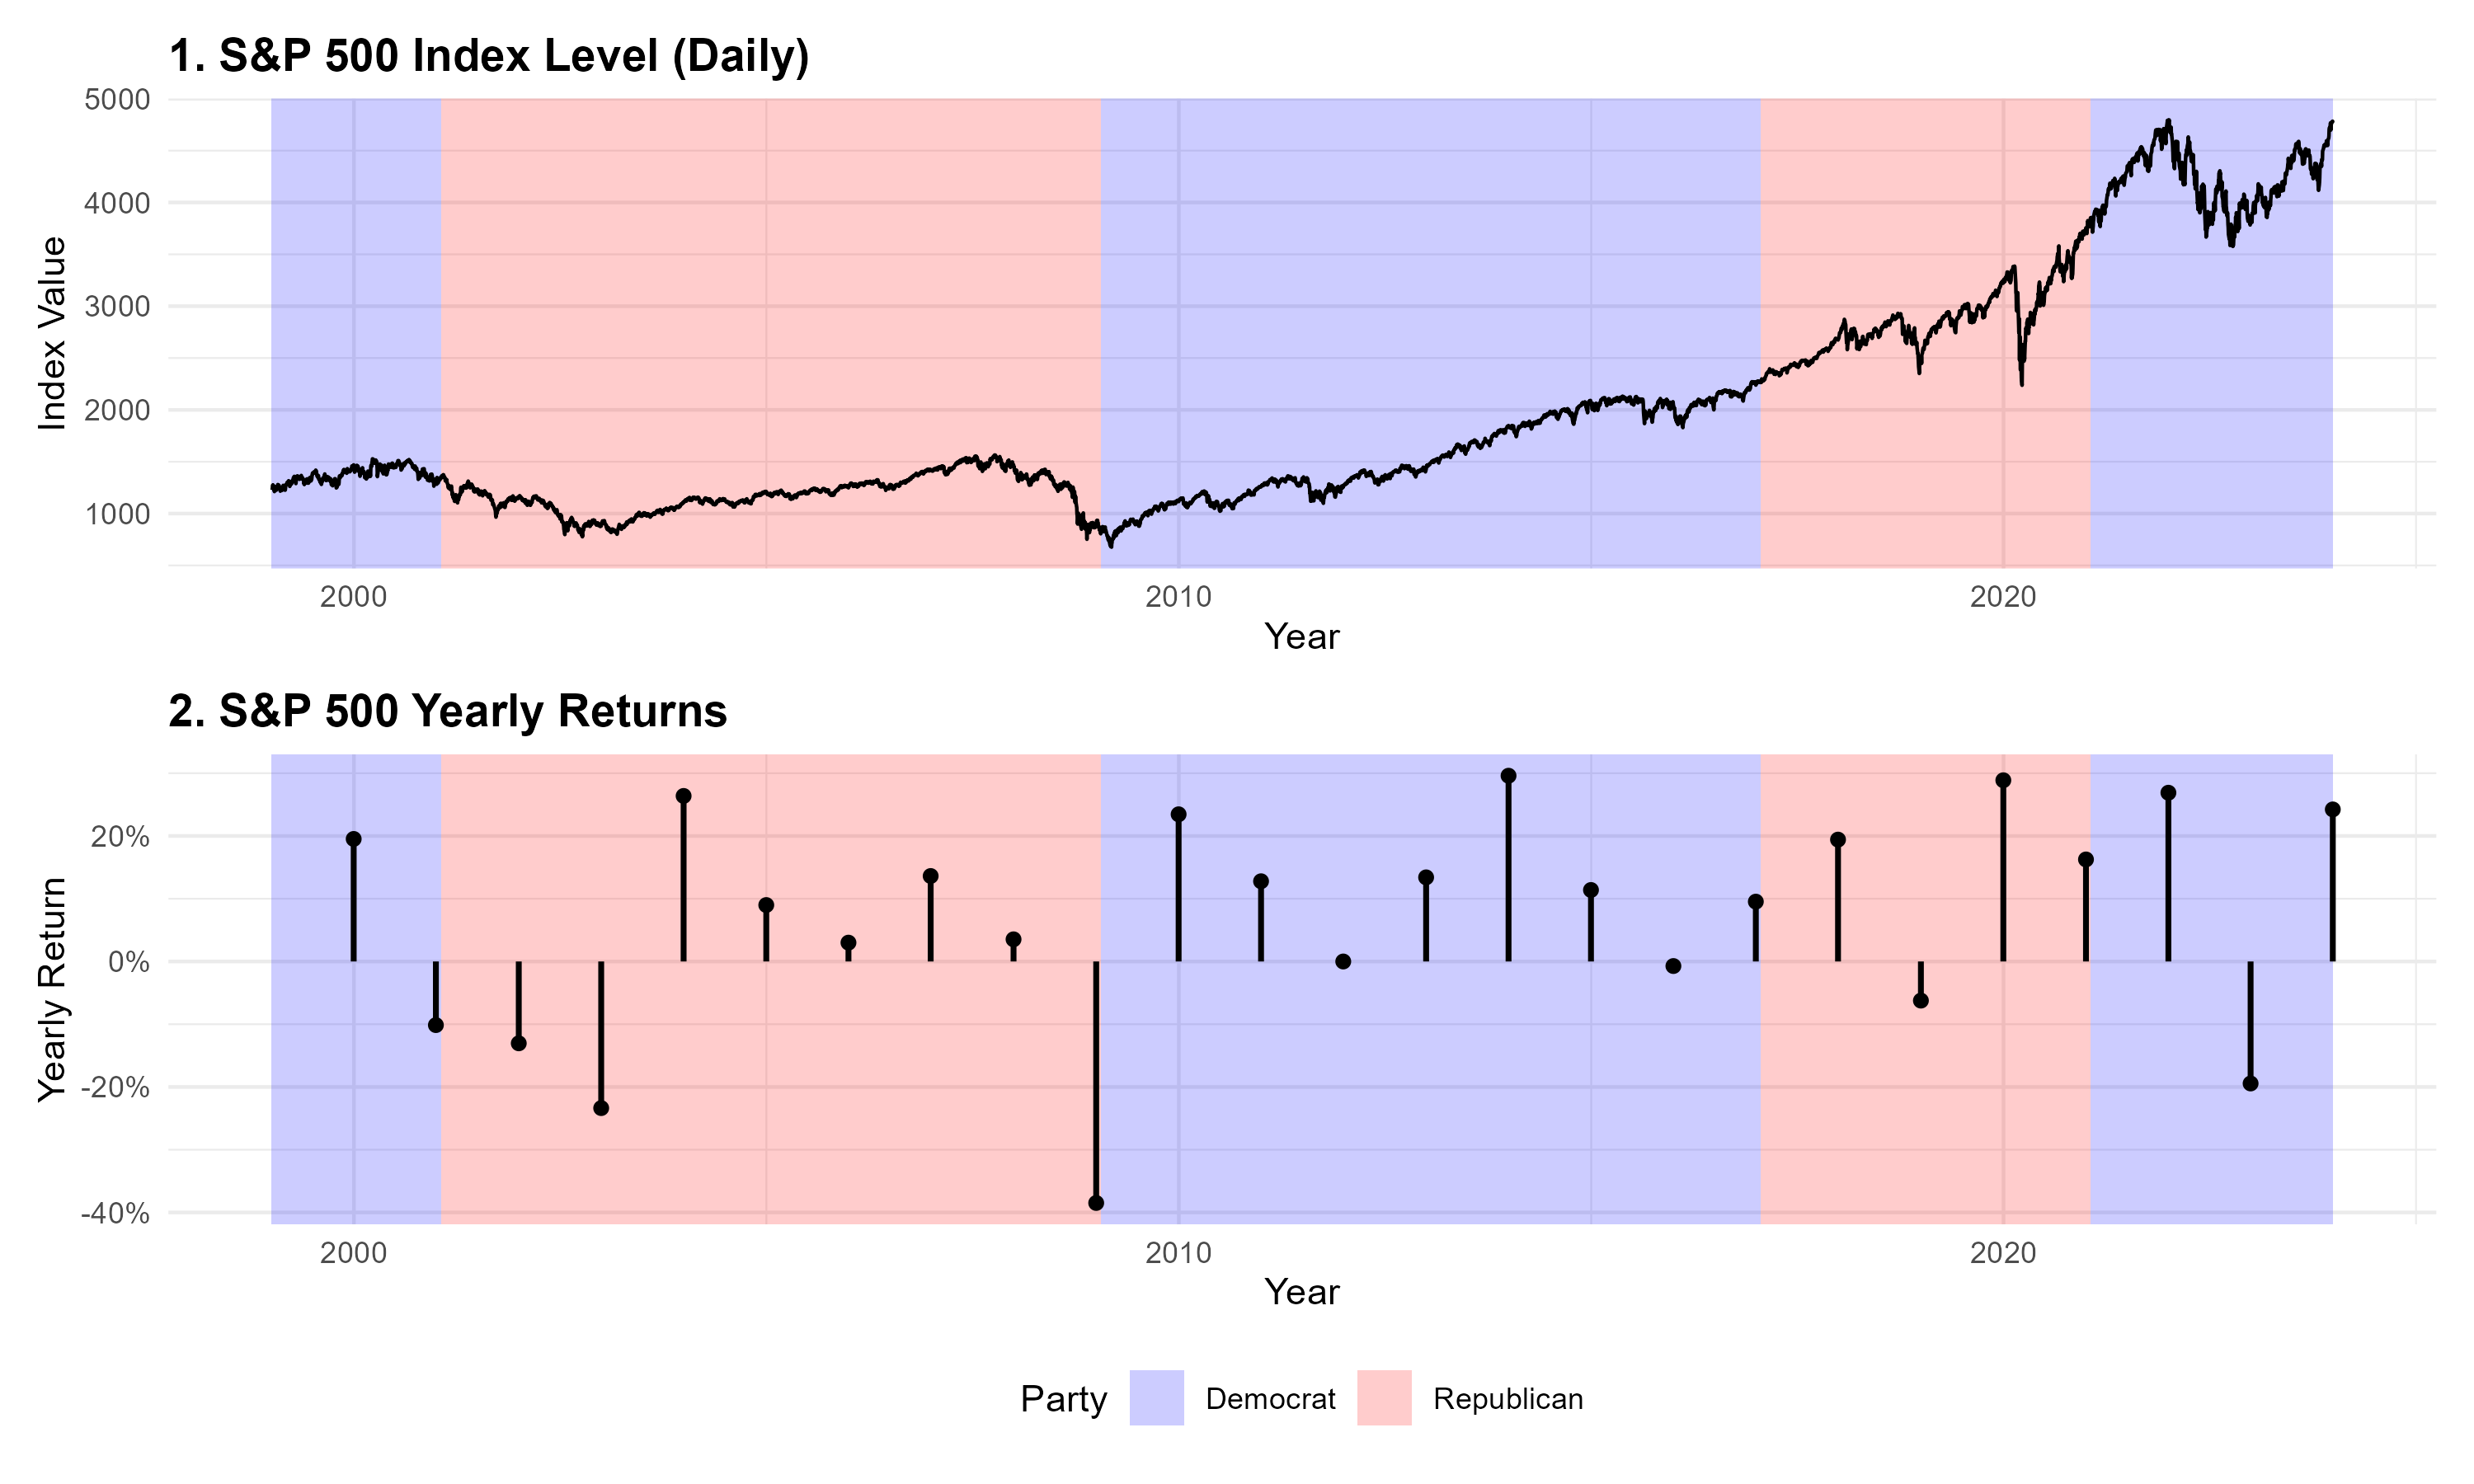
\includegraphics[width=\textwidth]{./figures/sp500.png}
    
    \begin{minipage}{\textwidth}
        \footnotesize This figure illustrates the historical performance of the S\&P 500 index throughout the sample period 1999-2023, overlaid with the corresponding U.S. presidential administrations. The top panel shows the the daily closing index value. The bottom panel marks the annual returns at the year-end. For example, the return plotted at 2000 represents the return from the end of 1999 to the end of 2000. The vertical background shading serves as a visual timeline for the federal political environment. Light blue shading designates periods during which the presidency was held by a Democrat, while the light red shading designates periods during which the presidency was held by a Republican.
    \end{minipage}
\end{figure}



\Cref{fig:sp500} illustrates the performance of the S\&P 500 index throughout the sample period, overlaid with the corresponding U.S. presidential administrations. The vertical background shading serves as a visual timeline for the federal political environment. The sample period encompasses both the dot-com bubble collapse and the Global Financial Crisis (GFC), both of which occurred during a Republican presidency. As illustrated by the S\&P 500 Yearly Returns chart, these periods are marked by severe negative market contractions, including a near -40\% yearly return drop in 2008, perfectly overlapping with the Republican-shaded timeline.

Conversely, the subsequent post-GFC bull market occurred during a Democratic presidency. The daily S\&P 500 index level shows a steady, prolonged upward trajectory during this Democrat-shaded period from roughly 2009 to 2017, accompanied by consistently positive yearly returns. Because these severe macroeconomic shocks and subsequent recoveries correlate so strongly with the alternating federal administrations in this specific timeframe, the FEDIR variable likely captures the mechanical suppression of stock market participation caused by these broader economic crises rather than a direct political effect.

Ultimately, this initial glance at the alignment data can be misleading if interpreted as a behavioral shift. As established in the direction reconciliation analysis, the aggregated state alignment variable is not a direct proxy for individual political preferences. Therefore, the lack of a significant state-level alignment effect is not a contradictory result to established literature, but rather a reflection of macroeconomic time-series variation and the limitations of ecological aggregation.


